
\documentclass[sigconf]{acmart}
\usepackage{graphicx}

%%
%% \BibTeX command to typeset BibTeX logo in the docs
\AtBeginDocument{%
  \providecommand\BibTeX{{%
    Bib\TeX}}}

%% These commands are for a PROCEEDINGS abstract or paper.
\acmConference[Usable Security \& Privacy Workshop]{May 2024}{Tel Aviv University}
%%
%%  Uncomment \acmBooktitle if the title of the proceedings is different
%%  from ``Proceedings of ...''!
%%



%%
%% Submission ID.
%% Use this when submitting an article to a sponsored event. You'll
%% receive a unique submission ID from the organizers
%% of the event, and this ID should be used as the parameter to this command.
%%\acmSubmissionID{123-A56-BU3}

%%
%% For managing citations, it is recommended to use bibliography
%% files in BibTeX format.
%%
%% You can then either use BibTeX with the ACM-Reference-Format style,
%% or BibLaTeX with the acmnumeric or acmauthoryear sytles, that include
%% support for advanced citation of software artefact from the
%% biblatex-software package, also separately available on CTAN.
%%
%% Look at the sample-*-biblatex.tex files for templates showcasing
%% the biblatex styles.
%%

%%
%% The majority of ACM publications use numbered citations and
%% references.  The command \citestyle{authoryear} switches to the
%% "author year" style.
%%
%% If you are preparing content for an event
%% sponsored by ACM SIGGRAPH, you must use the "author year" style of
%% citations and references.
%% Uncommenting
%% the next command will enable that style.
%%\citestyle{acmauthoryear}


%%
%% end of the preamble, start of the body of the document source.
\begin{document}
\acmBooktitle{Usable Security
\& Privacy Workshop, TAU}

%%
%% The "title" command has an optional parameter,
%% allowing the author to define a "short title" to be used in page headers.

\title{Enhancing Healthy Eating Habits: Balancing Privacy and Accuracy in Food Consumption Data Utilization}
\author{Lior Belenkov, Maya Iwanir}
\date{May 2024}

%%
%% The "author" command and its associated commands are used to define
%% the authors and their affiliations.
%% Of note is the shared affiliation of the first two authors, and the
%% "authornote" and "authornotemark" commands
%% used to denote shared contribution to the research.


%%
%% By default, the full list of authors will be used in the page
%% headers. Often, this list is too long, and will overlap
%% other information printed in the page headers. This command allows
%% the author to define a more concise list
%% of authors' names for this purpose.
\renewcommand{\shortauthors}{}

%%
%% The abstract is a summary of the work to be presented in the
%% article.
\begin{abstract}
Our main goal is motivating healthy eating, by collecting nutritional data while ensuring privacy. 
We will utilize a locally differentially private algorithm, which perturbs user data before it is sent to the data curator, and allows to estimate the average of the aggregated data. \\
 We compared how altering various parameters- such as the privacy budget epsilon, impacts privacy and accuracy metrics. Using the conclusions, we addressed the accuracy and privacy issues caused by collecting multiple nutritional values for each user. We examined the trade-offs for specific privacy and accuracy levels. The preferred levels will be determined through a user study, which will assess them based on the participants' concerns about data collection. 
\end{abstract}

%% This command processes the author and affiliation and title
%% information and builds the first part of the formatted document.
\maketitle

\section{Introduction}
Many companies collect user data, and users are unaware of how much their data reveals their behavior. The companies use the data to increase their profit, whether by selling it or publishing it \cite{riederer2011sale}.\\
Our goal is to motivate healthy eating habits in workplaces, and a major part of this initiative involves collecting telemetry data. We want the data to effectively represent the eating habits of the population, while also preserving the privacy of individual users.\\
To achieve this, we are going to use Local Differential Privacy- LDP, which is an algorithm that works directly on the user's device. On one hand, it hides the real data of each user before it is sent to the database. On the other hand, the overall aggregated privatized data reflect quite precisely the actual data.
\section{Background and Related Work}
Differential Privacy (DP) is a technique that provides privacy guarantees for users when collecting and analyzing their data. The centralized model requires a trusted data curator, as the privatization occurs after the data collection. We aim to provide a stronger privacy guarantee, which does not depend on a trusted third party. That's why we opted to use LDP- it ensures the privacy of user data throughout each step of the process, including the transmission of the data to the curator \cite{1_dwork2014algorithmic}.\\
An algorithm is considered $\epsilon$-LDP, if it maps from domain B to range C, such that for every two elements b, b' in B, and every subgroup- S of the range: $Pr\left[A(b)\in S\right] \leq e^{\epsilon}Pr\left[A(b')\in S'\right]$.\\ This definition promises, that the probability of a specific result originating from one input, is almost equal to the probability of it originating from any other input, when a suitable epsilon is chosen \cite{2_ding2017collecting}. We chose to focus on a specific implementation of LDP, known as Symmetric Unary Encoding- SUE \cite{3_wang2020comprehensive}.\\
Let's denote the number of users by N, and the number of timestamps for data collection (for each mean estimation) by L. We would like to evaluate the average of the collected user data, over the entire period. \\\\
Assumptions: Each input belongs to a continuous value range, from m to M. To limit the possible results, we group small ranges of values into buckets. The number of buckets is denoted by d, and the buckets are denoted by $\{B_i\}_{i=0}^{d-1}$. The range size is determined by d, which we will refer to as g (granularity level): $g=\frac{M-m}{d}$. Each user input belongs to a specific bucket and is represented by a d-bit histogram, with 1 in its bucket index and 0 in other indexes.\\
The algorithm privatizes the histogram, producing a d-bit vector. Using the privatized results, we can evaluate the sum of the original histograms from the users. Afterward, we calculate the mean of the privatized histograms and use it to estimate the original mean \cite{2_ding2017collecting}.\\\\
From the sequential composition theorem, we know an algorithm M, which is composed of a sequence of k $\epsilon$-LDP algorithms, is $k\cdot\epsilon$-LDP \cite{4_arcolezi2022improving}. We need to collect k values from each user, which are correlated. If there is a strong correlation between the values (for example- knowing one value reveals a different value), running an $\epsilon$-LDP algorithm on each value, can be equivalent to running an $\epsilon$-LDP algorithm k times on the same value. To guarantee $\epsilon$-LDP, we have to run an $\frac{\epsilon}{k}$-LDP algorithm on each value instead (known as Spl \cite{4_arcolezi2022improving}).\\
In our case, we aim to collect 3 nutritional values- such as carbs, fat, and protein, which are correlated, while maintaining the privacy level of $\epsilon$=2. To have such $\epsilon$-LDP guarantee, we have to privatize each value with an $\epsilon^*= \frac{2}{3}$ LDP algorithm. This approach reduces the accuracy of the results, and we will later discuss various solutions for that. Moreover, we are aware that there is a correlation between the nutritional intakes of the same user on different days. Due to sequential composition, for similar reasons as above, we aim to avoid executing the algorithm on the same value. We will introduce a technique to avoid privacy guarantee loss, called memoization \cite{2_ding2017collecting}.
\section{Methodology} Our implementation is based on dBitFlip, shown in [2]. Let's denote the actual value that a user sent by t. The calculation of the bucket index where t belongs is as follows: $$i_t =  \begin{cases}
0 & \text{if $t<m$}\\
\left \lfloor{\frac{t-m}{g}}\right \rfloor & \text{if $m\leq t \leq M$}\\
d-1 & \text{if $t>M$}    
\end{cases}$$
It is represented by a d bit vector- $v=(v_0,v_1,…,v_{d-1})$ where\\ $v_i = \begin{cases} 1 & \text{if $i=i_t$}\\
0 & \text{else} \end{cases}$.
From this vector, we calculate the privatized vector- $\hat{v}=({\hat{v}}_0,{\hat{v}}_1,\ldots,{\hat{v}}_{d-1})$ \footnote{the dBitFlip algorithm is based on sub-sampling of buckets. As the number of sampled buckets becomes larger, the accuracy becomes higher, but the communication cost becomes more expensive. We chose the number of sampled buckets to be equal to the total number of buckets, to get the maximum accuracy.} where ${\hat{v}}_{i_t}\sim Ber\left(p\right)$,$\ {\hat{v}}_j \sim  Ber\left(q\right)$ for each $j\neq i_t$, and $p=\frac{e^\frac{\varepsilon}{2}}{e^\frac{\varepsilon}{2}+1},\hspace{1 mm} q=1-p$. This vector will be sent to the server once every timestamp and will be later used for aggregation.\\
The server collects data from N users during L timestamps. Our mission is to evaluate $V_k=\frac{\mathrm{\sum}_{N, L} v_k}{NL}$ (the average of original vectors, in index k). The server gets a data tensor- H in shape NxLxd, where the entry H(i,j,k) is ${\hat{v}}_k$ of the i'th user in the j'th timestamp. To evaluate $V_k$, we calculate ${\hat{V}}_k$ as follows \cite{3_wang2020comprehensive}: (*) $${\hat{V}}_k=\frac{\frac{\left(\sum_{i=0}^{N-1}\sum_{j=0}^{L-1}H\left(i,j,k\right)\right)}{NL}-q}{p-q}$$  
Each bucket gets a weight, that equals its mean value: \\
$w=(w_0,w_1,…,w_{d-1})$ where
 $w_i=m+g\cdot(i+0.5)$. The mean estimation is the result of the inner product $\left\langle\hat{V},w\right\rangle$.\\ \\
Memoization: as shown in \cite{2_ding2017collecting}, the memoization technique stores the user's previous responses- the original histogram and its privatized form (on the user device, not visible to the server). As described before, when the user inputs a new value, it is converted to a histogram. Before the privatization process, we first check if the histogram appears in the previous responses- if it does, we use its previous privatized form instead of privatizing it again. Otherwise, the process continues as usual, and before sending we store the result.

\section{Results} \subsection{Accuracy} We performed experiments regarding the accuracy of the algorithm we presented earlier. We measure the average divergence of the estimated mean from the actual mean, depending on the following parameters: epsilon, number of buckets, and number of timestamps (L).
In both experiments, N=500, m=0, M=100, number of repetitions=32. The generated data is distributed normally with $\mu=67$, std=10. Each graph's x-axis is epsilon values, and the y-axis is the average divergence (upon repetitions) of the estimated mean from the actual mean.\\ \\
In the first experiment (Figure 1), we compared the effect of changing the number of buckets- d on accuracy. We set L to be constant- 7. We generate the data once and privatize it again for each repetition. Each graph represents a different number of buckets. It is evident that a reduced number of buckets is associated with improved accuracy, indicated by a smaller divergence. The slope of the graphs decreases as epsilon increases. We observed that after a certain epsilon, the accuracy improvement almost diminishes across all 4 graphs. For instance, in this current setting, it occurs at epsilon=2.
\\\\
In the second experiment (Figure 2), we compare the effect of changing the number of timestamps on accuracy. We set d to be constant- 20. For each repetition, we generate new data with the same distribution (because the number of timestamps changes), and privatize it. Each graph represents a different value of L. It is clear that increasing the number of data collection timestamps, leads to improved accuracy, as evidenced by reduced divergence. The slope of the graphs becomes smaller as the epsilon increases, leading to a decreased accuracy improvement.  In our current configuration, the slope diminishes after epsilon= 3 across all 4 graphs. Generally, we observe that after a certain value of L, further increasing this parameter only yields minimal accuracy improvement. In our case, the two lower graphs (L=21, L=28) are nearly identical. Selecting L=21 is the preferred option, because it is more usable for analysis, and the improvement from increasing L is minimal.\\ 
If we collect multiple nutritional values from each user, we need to adjust some parameters to achieve the same privacy guarantees and similar accuracy. Our experiments have shown that increasing L or decreasing d achieves this. The first solution raises the communication cost, and the second one compromises privacy (as we will explain in the next part). Therefore, the best practice is to combine them. Alternatively, increasing the number of participating workers (N) achieves the same effect, based on the estimation equation (*).
\begin{figure}[h]
    \centering
    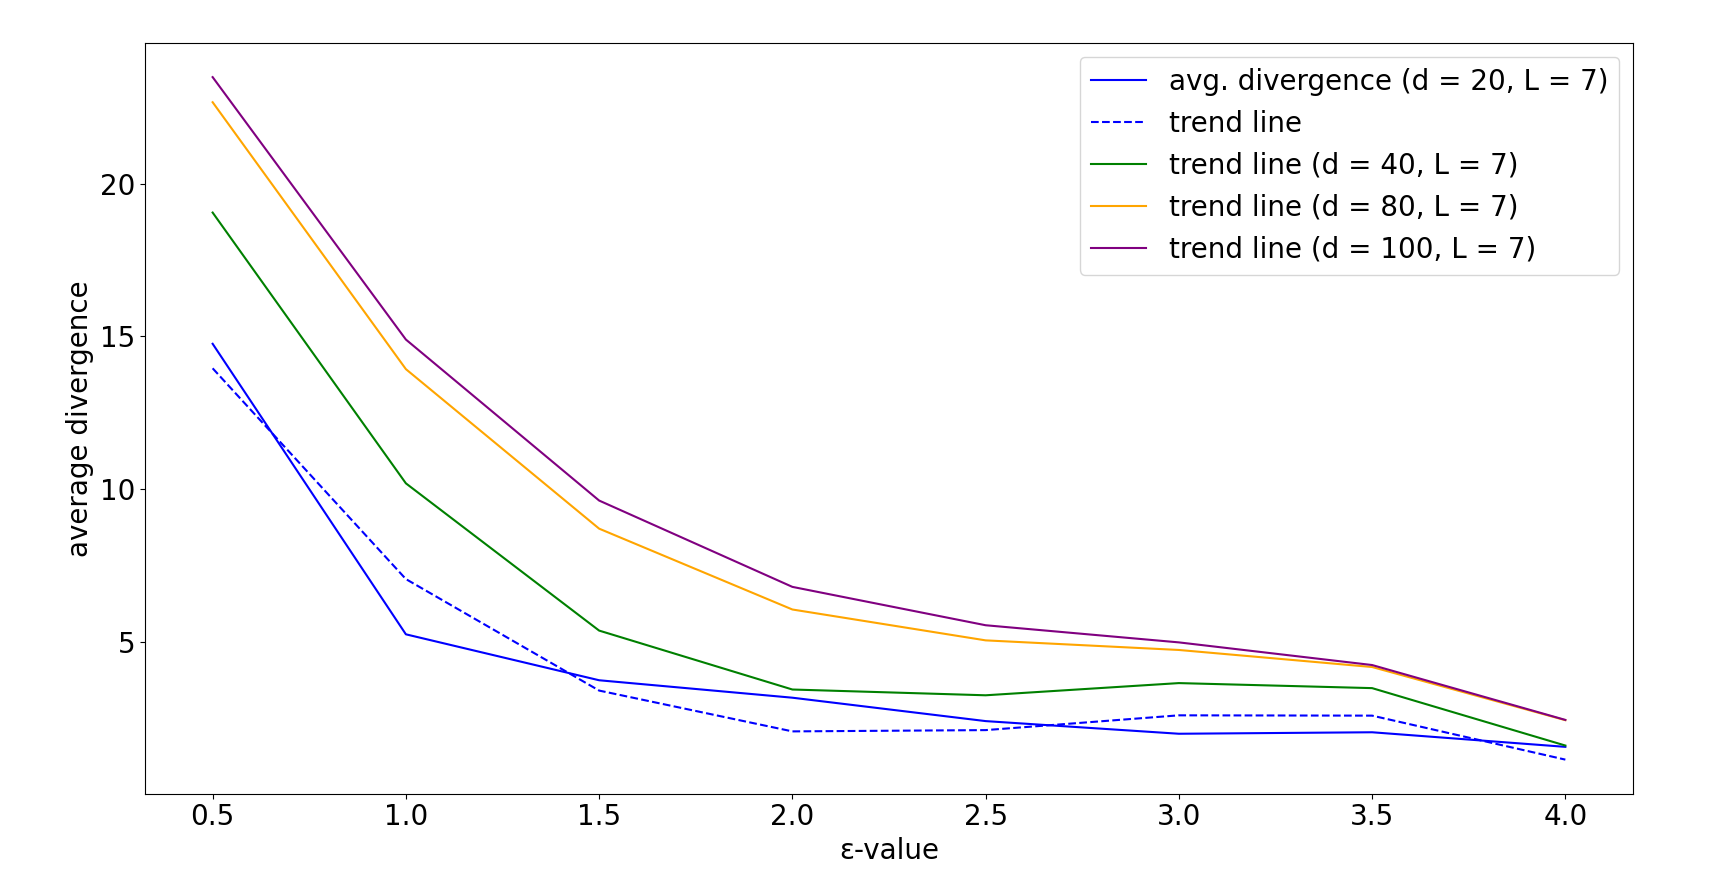
\includegraphics[width=.5\textwidth]{images/accuracy- d(3).png}
    \caption{Accuracy- number of buckets (d)}
    \label{fig:accuracy-d}
\end{figure}
\begin{figure}[h]
    \centering
    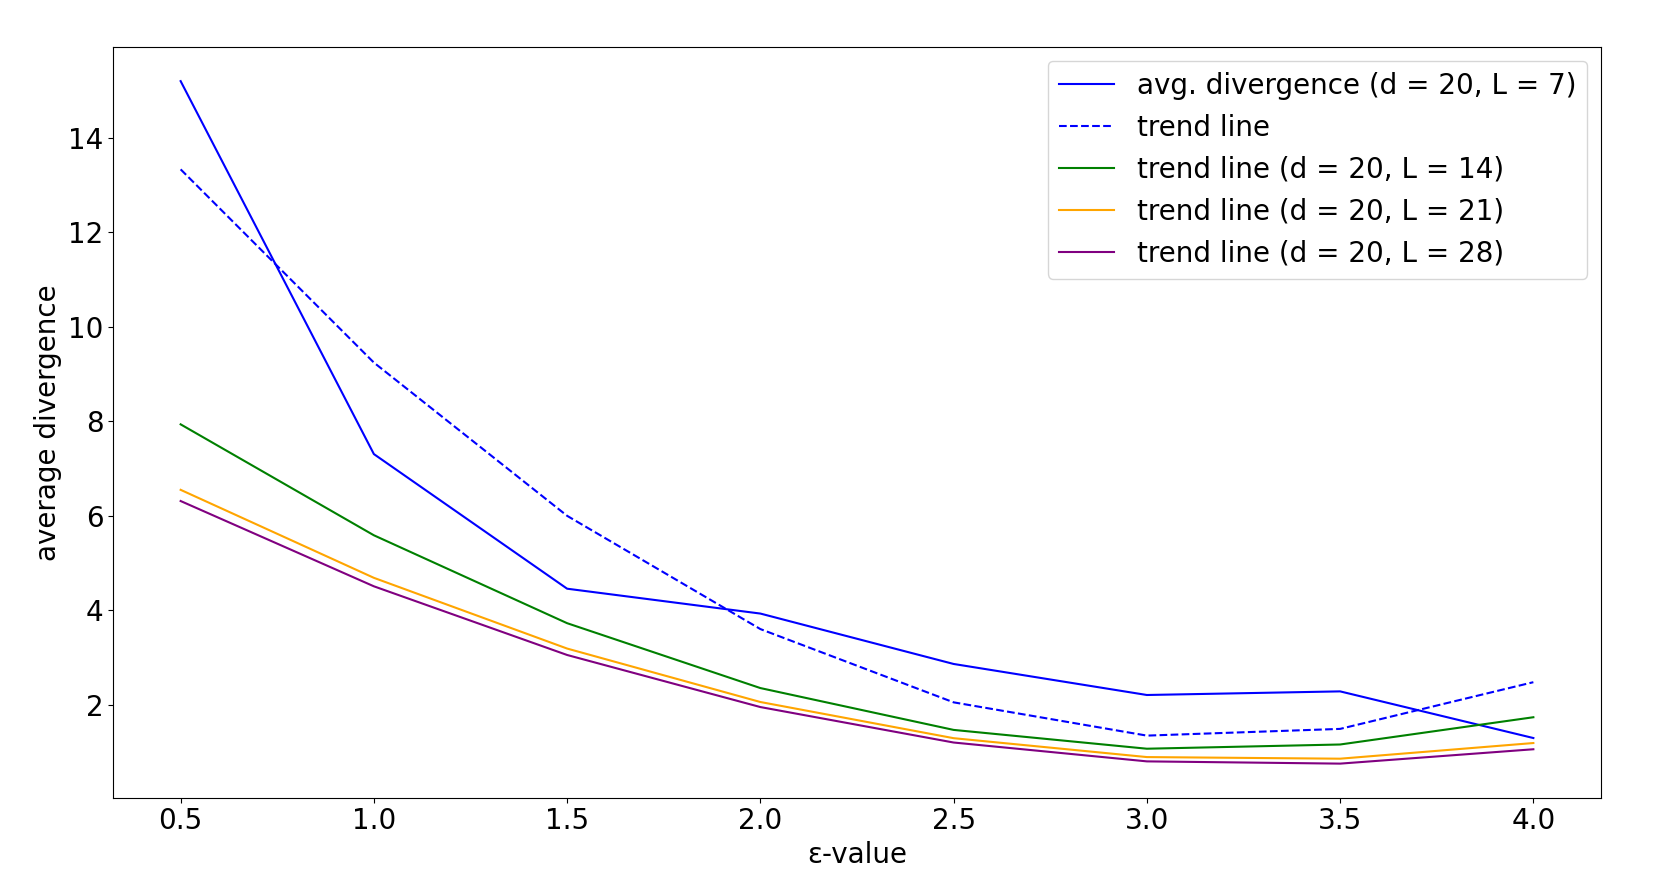
\includegraphics[width=.5\textwidth]{images/accuracy- L.png}
    \caption{Accuracy- number of timestamps (L)}
    \label{fig:accuracy-L}
\end{figure} 

\subsection{Privacy}  We performed different experiments regarding the privacy aspect of the algorithm. Given a privatized vector $\hat{v}$, we want to measure how "easy" it is to guess the original value from it. The probability that $\hat{v}_{i_t} =1$ is higher than the probability that $\hat{v}_{j} =1$ for $j \neq i_t$ (recall that $i_t$ is the bucket index where the original value belongs). Therefore, the optimal guessing technique w.o. prior knowledge, is to pick randomly (with the same probability) one of the indexes i where $\hat{v}_{i} =1$. In both experiments, the y-axis represents the average percent of correct guesses upon $2^{8}$ repetitions. As in the previous part, m=0, M=100, and the data distributes normally with $\mu=67$, std=10. \\\\
In the first experiment (Figure 3), the x-axis represents the epsilon value, and each graph represents a different number of buckets (d). We observe that all the graphs show an upward trend, indicating more correct guesses as epsilon grows larger. When comparing the graphs, we notice that decreasing d corresponds with more correct guesses, and therefore weaker privacy. Notice that increasing the value of d is a viable option to achieve a lower value in our metric, as the privacy improvement is noticeable even at higher values of d. As demonstrated in the accuracy experiments, higher values of d can impair accuracy. Therefore, it's important to consider the trade-off between privacy and accuracy.
\\\\
In the second experiment (Figure 4), the x-axis represents d, and each graph represents a different epsilon. The trend of all graphs shows a decrease in accuracy as the number of buckets becomes larger, as seen in the previous figure. Among the graphs, we can observe that smaller epsilon values correspond with better accuracy (as expected, according to the LDP definition). Generally, after a certain d value, the slope decreases significantly. Therefore, for each epsilon, increasing d beyond this value will not improve privacy as much. Moreover, we notice that after a specific value of epsilon, the privacy improvement diminishes. Specifically, in this case, between epsilon=0.5, epsilon=1, and epsilon=2 (after d=40) there is no significant difference, so the preferred option in terms of accuracy is epsilon=2.
    
\begin{figure}[h]
    \centering
    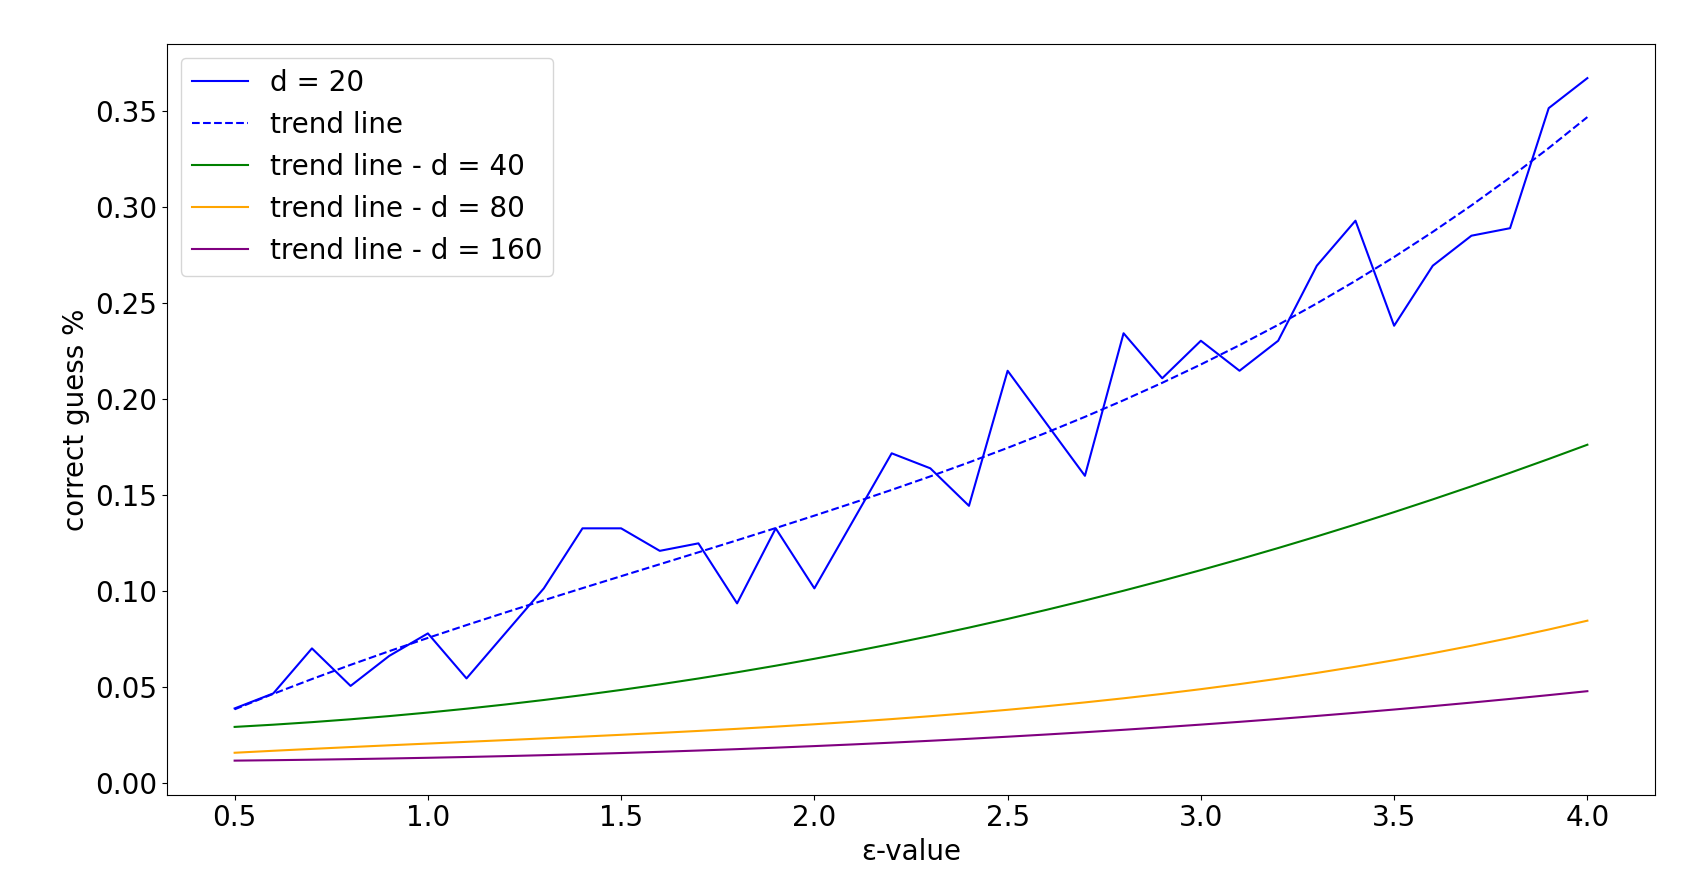
\includegraphics[width=.5\textwidth]{images/privacy- d.png}
    \caption{Privacy- number of buckets (d)}
    \label{fig:privacy-d}
\end{figure} 
\begin{figure}[h]
    \centering
    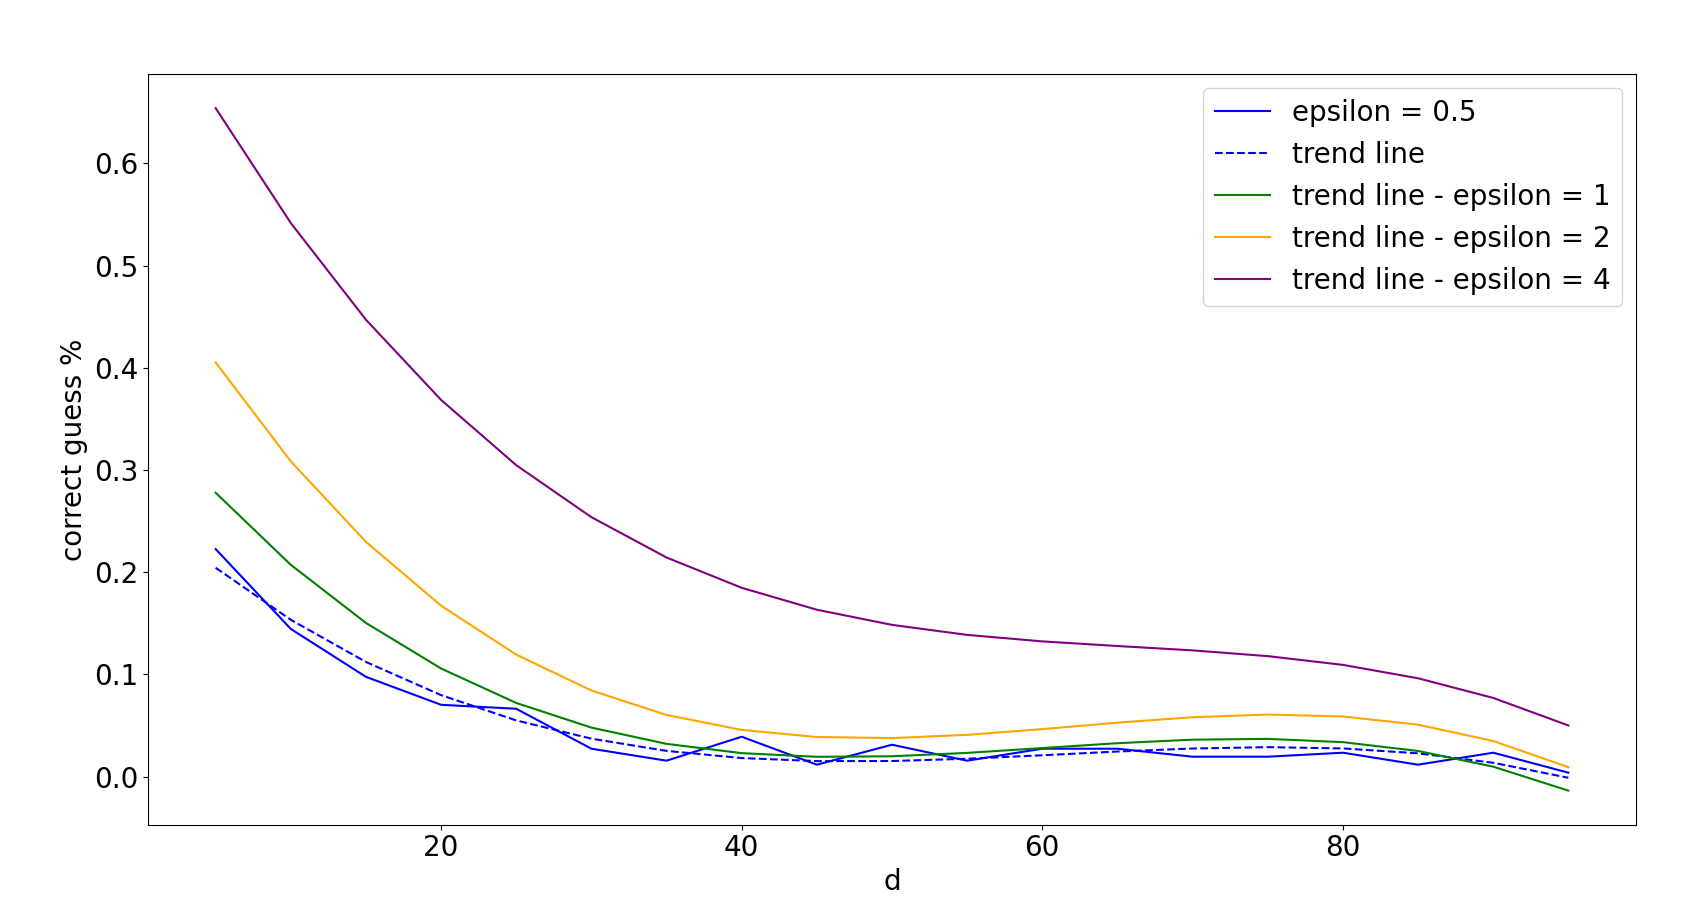
\includegraphics[width=.5\textwidth]{images/privacy- epsilon.png}
    \caption{Privacy- epsilon value ($\epsilon$)}
    \label{fig:privacy-epsilon}
\end{figure} 

To conclude this part, we saw that increasing the number of buckets can enhance privacy, measured in correct guesses, rather than solely decreasing epsilon. Without prior knowledge, this metric is useful to analyze the LDP mechanism. However, with prior knowledge, the guessing tactic we presented is sub-optimal, and a different metric should be considered. Through the user study, we will receive preferred levels of privacy and accuracy. We can achieve those levels by changing both the epsilon and the number of buckets.

\section{Discussion}

 By presenting results and implementing the LDP mechanism in an accessible and publicly available package, we look forward to increase awareness and credibility for private data collection options.

\subsection{Limitations} As present, the mechanism we are using provides an estimate of the average histogram, enabling us to calculate the mean and approximate the distribution. However, there are other statistical measures that interest us, such as the median, which may be unattainable through our current mechanism and may require a different approach.

\begin{figure}[h]
    \centering
    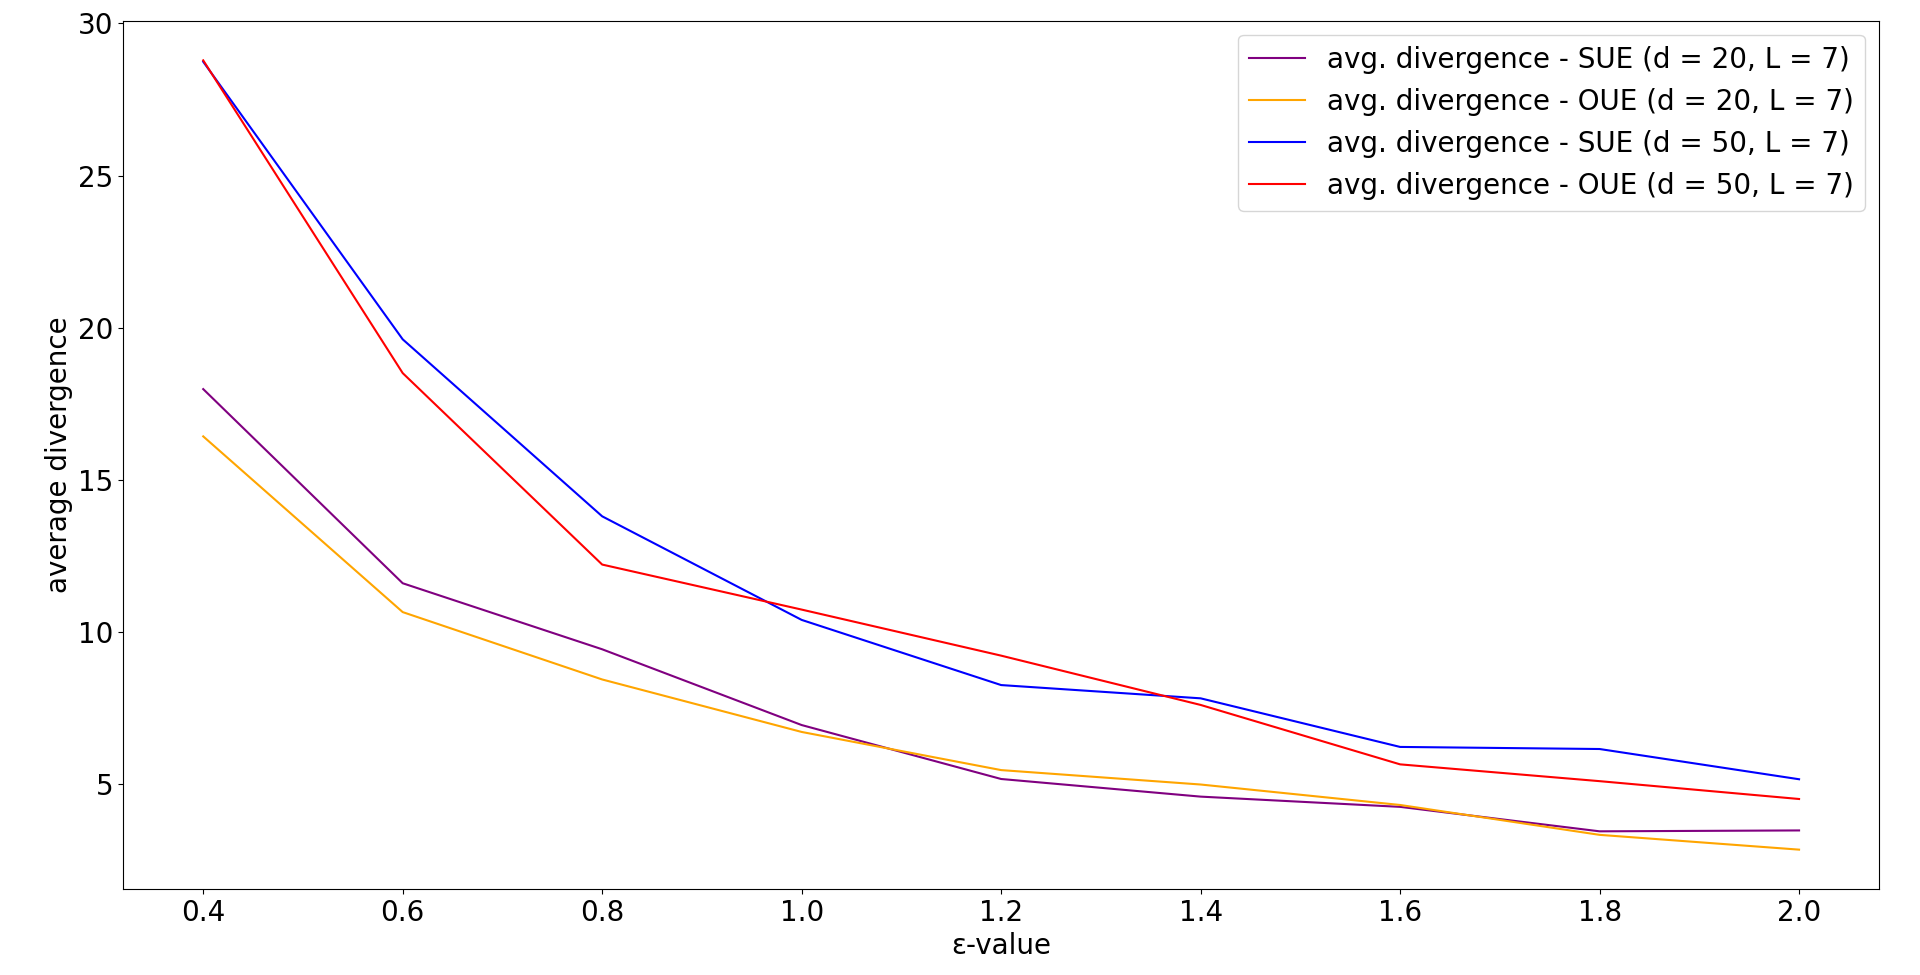
\includegraphics[width=0.5\textwidth]{images/SUE OUE.png}
    \caption{Accuracy- SUE vs OUE}
    \label{fig:enter-label}
\end{figure}
\begin{figure*}[ht]
    \begin{center}
        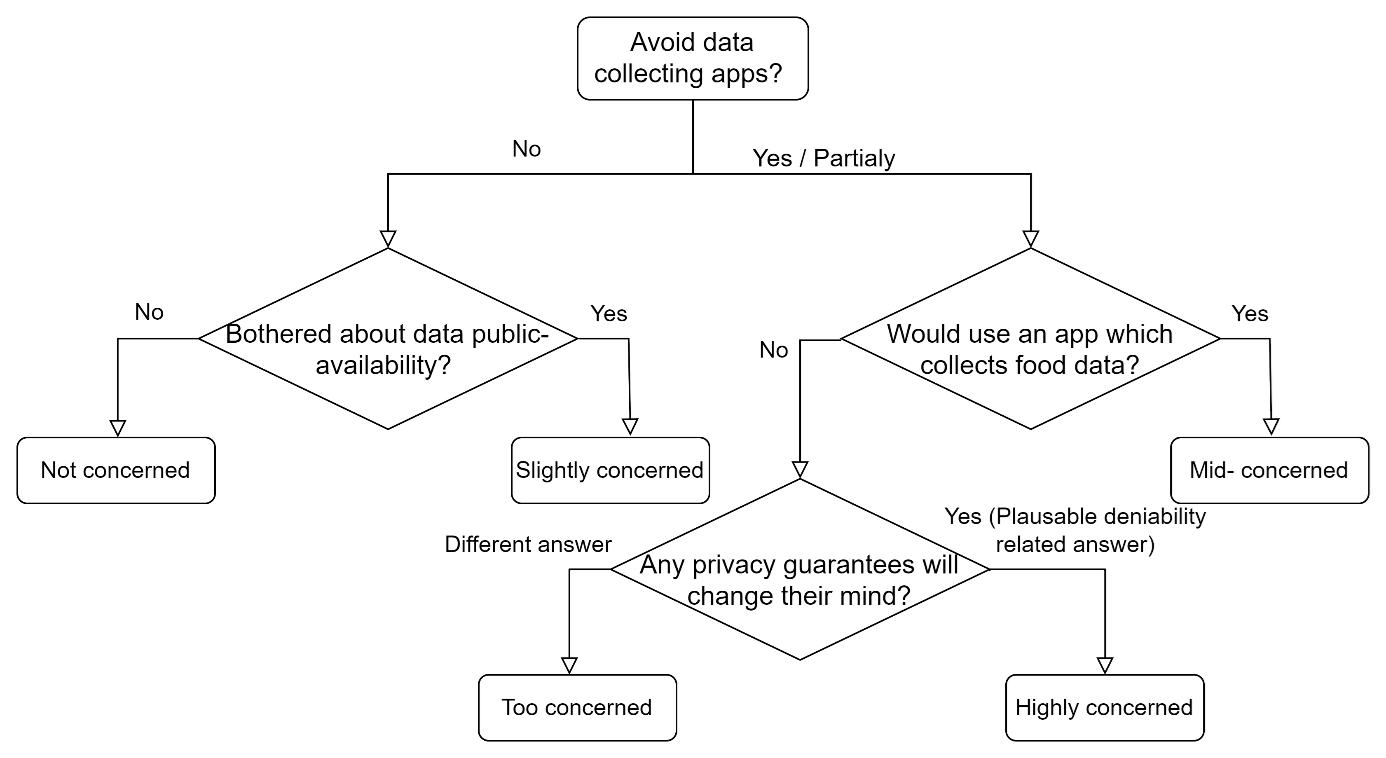
\includegraphics[width=\textwidth]{images/classification.png}
        \caption{Classification of users}
        \label{fig:accuracy-d}
    \end{center}
\end{figure*} 
\subsection{Future work} There are numerous LDP mechanisms, some of which may improve the estimation. Optimized Unary Encoding (OUE), is a different unary encoding approach, that minimizes the variance of UE \cite{3_wang2020comprehensive}. The only difference between the implementation of SUE and OUE are the probabilities p and q in the privatization process: for OUE they are $p=\frac{1}{2}$ and $q=\frac{1}{e^{\epsilon}+1}$. We compared the accuracy of both methods in the following settings: N=500, L=7, m=0, M=100, and number of repetitions=128. The generated data is distributed normally with $\mu=67$, std=10. We observe (Figure 5) that in both settings- d=50 and d=100, there is no significant difference between the average divergence of SUE and OUE. Therefore we chose to stick to SUE.\\
Another technique that may provide better estimation when collecting multiple values is Smp, which is based on uniformly sampling only one value from each user and assigning the original privacy budget to it \cite{4_arcolezi2022improving}. According to the article, the results of this method are more accurate than the results of Spl. We were interested in measuring the improvement in accuracy by changing the parameters d and L. We chose Spl for a more straightforward analysis. However, our data is limited, and it might be worth testing these methods once we collect more authentic data, and reconsider.

\subsection{User Study} In order to select the appropriate epsilon for our app, we will be conducting a user study. The main objective of the study is to fit the company's preferences- in terms of privacy and accuracy.
The user study protocol we have designed, is specifically directed to the company's employees, who will be required to share data about the food they eat to use the app. Therefore, the study is focused on the privacy aspect. We can design a similar study for the company's management, focusing more on the accuracy aspect. The study is divided into 3 parts:
\subsubsection{Part 1:}  Classification of the users by the importance of privacy to them. The classification will determine the weight of the answers about the level of privacy- "highly concerned" users will get the highest weight (3), "mid-concerned" users will get a smaller weight (2), and "slightly concerned" users will get the smallest weight (1). Users who classify as "not concerned" or "too concerned" will get a weight of 0- they are either indifferent to privacy, or care too much about it to be a potential user (respectively).
The diagram in Figure 6 demonstrates the classification process.
\subsubsection{Part 2:} Willingness to share data under our privacy mechanism, using different epsilons. First, we explain our app and the importance of privacy and accuracy. We then provided an intuitive explanation of the mechanism we use, along with the impact of the privacy parameter epsilon. The explanation simplifies the mechanism enough, so the user can make reasonable choices about epsilon \cite{5_nanayakkara2023chances}. The epsilon choices we gave were: 0.5, 1, 1.5, 2, 2.5, 3, 4. For each epsilon, we wrote the expected number of buckets with the value 1 after the privatization, out of 100 buckets. We calculated them using the following formula, which derives from the probabilities p and q of the mechanism:  $100-\left(\frac{e^{\frac{\epsilon}{2}}}{e^{\frac{\epsilon}{2}}+1}\cdot99+\ \frac{1}{e^{\frac{\epsilon}{2}}+1}\right)$.\\
The users were asked to vote for each epsilon from 1- very unlikely to share, to 5- very likely to share.
\subsubsection{Part 3:} Rating accuracy levels. We gave the users various deviations of the results from the actual mean, with an example of mean = 37. They were asked to rate each deviation on a scale from 1 to 5, based on how well it reflects the actual mean in their opinion: 1- reflects very poorly, 5- a good reflector.\\
Finally, after collecting the the study's answers, we will rank the epsilons in the privacy part, and the deviations in the accuracy part, based on the responses and the users' classification (multiplying each answer by the weight in the accuracy part). The epsilon with the highest rank in the privacy section will be chosen, and we will select L and d based on the deviation with the highest rank. 

\section{Conclusion}
In this report, we analyzed average estimation in the Local Differential Privacy model. We have introduced and implemented the SUE LDP mechanism for single value data collection, together with the Spl technique for multiple values. With this implementation, we analyzed the privacy and accuracy using specific metrics.\\ We compared the effect of changing various parameters on those metrics, significantly enhancing our understanding of LDP.\\ Privacy improvement can be achieved by decreasing epsilon or increasing the number of buckets (d), and accuracy improvement can be achieved by decreasing d or increasing the number of timestamps (L). We considered the trade-off between the parameters to achieve the privacy and accuracy goals.

\section{Contributions}
We worked collaboratively on the report, the code and the demo implementation, as well as the user study protocol. \\
We would like to thank the course staff for their help in planning and constructing the project. 

%%
%% The next two lines define the bibliography style to be used, and
%% the bibliography file.
%%\bibliographystyle{ACM-Reference-Format}
\bibliographystyle{unsrt}
\bibliography{reference}

%%
%% If your work has an appendix, this is the place to put it.
\appendix


\end{document}
\endinput
%%
%% End of file `sample-sigconf-authordraft.tex'.
